This section specifies the software architecture requirements and the software
architecture design for web application framework.

\subsection{Architecture Requirements}
The web application framework provides the software architecture for the software
providing browser based access to human users.

\subsubsection{Access and Integration Requirements}
\paragraph{Access Channel Requirements}
The web application framework will address the first human access channel requirment
referred to in section \ref{sec:humanAccessChannelManagementSystem},
namely the requirement of human users of the system to access the application
via a web browser. The web application must be accessable to any user who uses
the latest version of any of the major bowsers namely Mozilla Firefox, 
Google Chrome, Apple Safari, Opera and Microsoft Internet Explorer.

\paragraph{Integration Channel Requirements}
The web application must integrate with the management system in order to allow
users to derive value. However, the web application will integrate with the
business layer through the web services layer, allowing one to decouple the
business and presentation layers from one another. This assist in delivering on
the required performance, maintainability and flexability requirement set for
the system as a whole.

\subsubsection{Quality Requirements}
The most important quality requirements for the web application layer are
\paragraph{Usability}
As the system is build for human users, it is important that users using the
system feel as though the system delivers what they require when they
require it i.e. users should be allowed to derive the exact value they require
from the system, no more and no less.

\paragraph{Maintainability}
It is important that the system as a whole can be easily expanded, implying
that if the backend system is expanded the front-end should continue to function,
which will allow developers to update the frontend as required. For this reason
a modern JavaScript framework such as ReactJS was chosen to assist developers 
to maintain the system much easier, allowing the code base to mature with time
without losing strict control and structure.

\paragraph{Performance}
ReactJS improves upon the work of earlier frameworks such as AngularJS which both
users and developers felt to be slow, because of the way in which monitoring of
bounded data was implemented. With ReactJS being built from the ground up with a
focus on user expierence from Facebook Inc., a much friendlier and faster framework
was developed, with significant performance increase seen from earlier frameworks.

	
\subsubsection{Architectural Responsibilities}
The architectural responsibilities of the Web Application Framework are shown in 
Figure \ref{fig:webApplicationFrameworkResponsibilities}
\begin{figure}[H]
	\begin{center}
	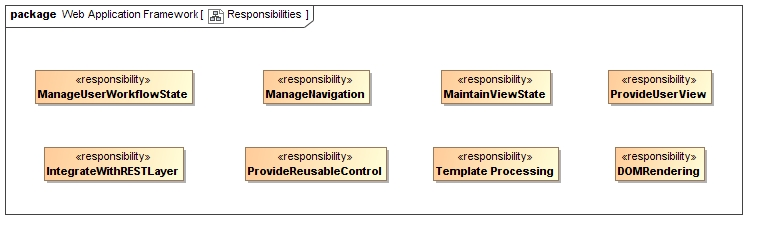
\includegraphics[scale=0.35]{../Diagrams and Charts/Web Application Framework/Responsibilities.jpg}
	\caption{The architectural responsibilities of the Web Application Framework}
	\label{fig:webApplicationFrameworkResponsibilities}
	\end{center}
\end{figure}

\subsection{Architecture Design}
This section specifies the very high-level software architecture design, i.e.
the software architecture design for the top level of granularity. Including 
allocation of architectural responsibilities to architectural components, any
tactics which should be used at the current level of granularity to address
quality requirements.

\subsubsection{Tactics}
Tactics which should be used to address the quality requirements should include:
\begin{itemize}
	\item caching of pre-generated and pre-populated HTML pages for performance
	\item virtual DOM for in-memory updates, incremental builds and efficient 
	diffing based on differentiation between static and dynamic DOM elements
\end{itemize}
\subsubsection{Architectural Components}
The architectural components of the  Web Application Framework are shown in Figure \ref{fig:webApplicationFrameworkResponsibilityAllocation}
\begin{figure}[H]
	\begin{center}
	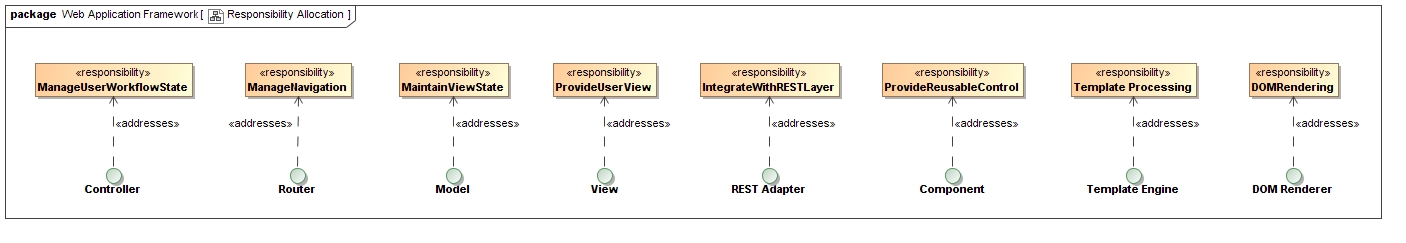
\includegraphics[scale=0.35]{../Diagrams and Charts/Web Application Framework/ResponsibilityAllocation.jpg}
	\caption{The abstract components to which the Web Application Framework responsibilities are assigned.}
	\label{fig:webApplicationFrameworkResponsibilityAllocation}
	\end{center}
\end{figure}

\subsubsection{Frameworks and Technologies}
The web framework will be based on \textbf{ReactJS}. ReactJS is an open-source web
application framework. The framework promises a model in which sub-components
cannot directly affect enclosing components.

Core reasons for using ReactJS:
\begin{itemize}
	\item The framework requires a defined structure which aids in maintainability.
	\item The framework is maintained not only by a community of users but also
	by Facebook and Instagram, this aids further in maintainability due to the 
	constant upkeep of documentation.
	\item The model supports integration with RESTful API services.
	\item Release of React Native which will allow for React based architecture 
	to native Android and iOS applications making the task of developing an 
	application, should time permit, easier.
\end{itemize}
Other frameworks were considered;
\begin{itemize}
	\item \textbf{AngularJS}: which is a powerful extensible framework with good modularization
, however, there is no consistent way to approach application development which may 
lead to difficulty regarding maintenance. The virtual DOM approach in ReactJS is more
efficient. Angular is also being replaced by ReactJS as the current standard for web 
application development and as a team with minimal experience in Angular we decided 
that we'd rather get experience in a future standard which is also easier to learn.
	\item \textbf{Ember.js}: 
	\item \textbf{Backbone.js}:
\end{itemize}

\paragraph{Concrete Realization of Architectural Components}
The concrete realization of components within \textbf{ReactJS} are shown in Figure
\paragraph{Tactics}
\paragraph{Tools}
\begin{itemize}
	\item Uses JavaScript so no need to learn another language/syntax.
\end{itemize}
\paragraph{Concepts and Constraints for Application Components}